% ============================================================================
% Municipality-Scale Flood Risk Mapping in Bolivar, Colombia
% Using Sentinel-1 SAR and Ensemble Machine Learning (2015--2025)
% Authors: Cristian Espinal Maya, Santiago Jimenez Londono
% Format: arXiv preprint
% ============================================================================

\documentclass{article}

\usepackage{arxiv}

\usepackage[utf8]{inputenc}
\usepackage[T1]{fontenc}
\usepackage{hyperref}
\usepackage{url}
\usepackage{booktabs}
\usepackage{amsfonts}
\usepackage{amssymb}
\usepackage{amsmath}
\usepackage{nicefrac}
\usepackage{microtype}
\usepackage{graphicx}
\usepackage{multirow}
\usepackage{siunitx}
\sisetup{
    group-separator = {,},
    group-minimum-digits = 4,
}
\usepackage{natbib}
\usepackage{tabularx}
\usepackage{textcomp}

\graphicspath{{./figures/}}

\title{Municipality-Scale Flood Risk Mapping in Bol\'ivar, Colombia, Using Sentinel-1 SAR and Ensemble Machine Learning (2015--2025)}

\author{
  Cristian Espinal Maya\thanks{Correspondence: cespinalm@eafit.edu.co. ORCID: \href{https://orcid.org/0009-0000-1009-8388}{0009-0000-1009-8388}} \\
  School of Applied Sciences and Engineering\\
  Universidad EAFIT\\
  Medell\'in, Colombia \\
  \texttt{cespinalm@eafit.edu.co} \\
  \And
  Santiago Jim\'enez Londo\~no\thanks{ORCID: \href{https://orcid.org/0009-0007-9862-7133}{0009-0007-9862-7133}} \\
  School of Applied Sciences and Engineering\\
  Universidad EAFIT\\
  Medell\'in, Colombia \\
  \texttt{sjimenez@eafit.edu.co} \\
}

\begin{document}
\maketitle

\begin{abstract}
We present a reproducible, open-access framework that delivers municipality-level flood risk statistics for all 46 municipalities of the Department of Bol\'ivar, Colombia (\SI{25978}{\kilo\metre\squared}; $\sim$2.2 million inhabitants)---one of the country's most flood-affected departments, encompassing the Depresi\'on Momposina, Canal del Dique, and La Mojana wetland systems. We processed 2,847 Sentinel-1 C-band SAR scenes (2015--2025) within Google Earth Engine using adaptive Otsu thresholding to produce 132 monthly water extent maps at \SI{10}{\metre} resolution. Eighteen predictor variables---with HAND thresholds relaxed for flat lowland terrain (flood label $<$\SI{10}{\metre}; non-flood $\geq$\SI{40}{\metre})---were integrated into a weighted ensemble of Random Forest, XGBoost, and LightGBM, achieving AUC-ROC $= 0.95 \pm 0.02$ under spatial five-fold cross-validation. HAND, SAR flood frequency, and distance to drainage were identified as dominant predictors via SHAP analysis. Overlaying the susceptibility surface with \SI{100}{\metre} population data reveals that approximately 580,000 people (26.4\% of the department) reside in high or very high susceptibility zones, concentrated in the Depresi\'on Momposina, the Mojana floodplain, and the Canal del Dique corridor. La Ni\~na years amplified mean flood extent by 41\% relative to El Ni\~no years ($p < 0.001$). The entire framework is open-access and fully reproducible (\url{https://github.com/Cespial/bolivar-flood-risk}).
\end{abstract}

\keywords{flood susceptibility mapping \and Sentinel-1 SAR \and ensemble machine learning \and HAND \and Google Earth Engine \and SHAP \and ENSO \and population exposure \and Bol\'ivar Colombia \and Depresi\'on Momposina \and Caribbean lowlands}

%%%%%%%%%%%%%%%%%%%%%%%%%%%%%%%%%%%%%%%%%%
\section{Introduction}
\label{sec:introduction}

Between November 2010 and May 2011, a La Ni\~na event struck Colombia with exceptional intensity: over 300 people died, 2.3 million were displaced, and direct losses exceeded USD 7.8 billion \citep{Hoyos2013}. The Department of Bol\'ivar was the most affected department nationally, with approximately 60,000 households impacted---yet municipal governments operated with national-scale hazard maps that could not distinguish which floodplain corridors, ci\'enagas, or levee-protected areas had been inundated. Fifteen years later, most of Bol\'ivar's 46 municipalities still lack the spatially explicit flood information mandated by their own planning instruments.

Globally, flooding affects approximately 1.65 billion people per decade \citep{UNDRR2020}. \citet{Tellman2021} showed that population exposure to flooding grew 20--24\% between 2000 and 2018, while \citet{Rentschler2022} estimated 1.81 billion people in significant flood hazard zones, 89\% in low- and middle-income countries. However, a persistent disconnect separates the scale at which satellite-derived flood products are generated (continental or national) from the scale at which flood risk decisions must be made (municipal) \citep{Bates2023}. This mismatch is acute in Colombia, where Ley~1523 of 2012 decentralizes flood risk management to municipalities, each legally mandated to formulate a Plan de Ordenamiento Territorial (POT) and a Plan Municipal de Gesti\'on del Riesgo de Desastres (PMGRD) \citep{CongresoCol2012}. Yet most lack the technical capacity to produce the required geospatial inputs \citep{OECD2019}.

Three technological developments now converge to address this gap. First, Sentinel-1 SAR provides cloud-penetrating imagery at \SI{10}{\metre} resolution with 6--12 day revisit, overcoming the $>$70\% cloud contamination that renders optical sensors ineffective in tropical regions \citep{Twele2016, DeVries2020}. Second, ensemble machine learning (Random Forest, XGBoost, LightGBM) consistently outperforms traditional methods for flood susceptibility prediction \citep{Mosavi2018, Darabi2021}, with SHAP enabling model interpretability \citep{Lundberg2017}. Third, Google Earth Engine democratizes petabyte-scale satellite processing \citep{Gorelick2017}. Despite these advances, comprehensive frameworks carrying the analysis from raw SAR data through to municipality-level risk statistics remain rare, and the flood susceptibility ML literature is conspicuously underrepresented in Caribbean lowland environments \citep{FloodRiskLAC2022}.

Global flood hazard products---including Fathom Global (\SI{90}{\metre}), the Global Flood Database \citep{Tellman2021}, and JRC Global Surface Water \citep{Pekel2016}---have transformed continental-scale flood assessment. However, their spatial resolution precludes the delineation of ci\'enaga boundaries, canal levee failures, and urban-fluvial interfaces critical for municipal planning in departments like Bol\'ivar. Our municipal-scale framework is designed to be \textit{complementary}, not redundant: it ingests global products (JRC, MERIT Hydro) as input features while delivering locally actionable outputs at resolutions 3--9$\times$ finer than existing global layers.

\textbf{Research gap and contributions.} Existing flood susceptibility studies in tropical South America are either (a) site-specific ($<$\SI{1000}{\kilo\metre\squared}), precluding administrative-scale risk ranking, or (b) based on global products at \SI{90}{\metre}--\SI{250}{\metre} resolution that cannot resolve the complex flood dynamics of internally drained lowland systems like the Depresi\'on Momposina. No previous study has produced municipality-level flood risk statistics for Bol\'ivar---one of Colombia's most flood-affected departments---using high-resolution SAR data. This work makes three specific contributions: (1) a complete SAR-to-municipality pipeline processing Sentinel-1 scenes across \SI{25978}{\kilo\metre\squared} and 11 years, with threshold adaptations for flat Caribbean lowland terrain; (2) an ensemble ML susceptibility model validated through spatial cross-validation with SHAP-based interpretability; and (3) quantified population exposure at the municipal level for all 46 municipalities and 6 ZODES (Zonas de Desarrollo Econ\'omico y Social), producing outputs directly ingestible by Colombian POT and PMGRD instruments.

\subsection{Study Area}
\label{sec:study_area}

\begin{figure}[htbp]
\centering

\includegraphics[width=0.75\textwidth]{fig01_study_area.pdf}
\caption{Department of Bol\'ivar, Colombia, showing six ZODES subregions and 46 municipalities. The department spans from the Caribbean coast (Cartagena de Indias) to the Magdalena Medio interior.}
\label{fig:study_area}
\end{figure}

The Department of Bol\'ivar (\SI{25978}{\kilo\metre\squared}; 7\textdegree{}30'--10\textdegree{}48'\,N, 73\textdegree{}45'--75\textdegree{}42'\,W) comprises 46 municipalities organized into six ZODES subregions (Figure~\ref{fig:study_area}), with approximately 2.2 million inhabitants \citep{DANE2018}. Unlike the mountainous departments of the Andean interior, Bol\'ivar is predominantly flat lowland terrain: over 90\% of the department lies below \SI{200}{\metre} a.s.l. The landscape is shaped by four major river systems---the Magdalena (Colombia's principal artery, $\sim$\SI{7000}{\cubic\metre\per\second} mean discharge at Calamar), the Cauca, the San Jorge, and the man-made Canal del Dique (\SI{115}{\kilo\metre} distributary from Calamar to the Bay of Cartagena) \citep{Restrepo2000, Restrepo2014}.

Three areas concentrate extreme flood vulnerability:

\begin{enumerate}
    \item \textbf{Depresi\'on Momposina}: An internal delta of $\sim$\SI{3400}{\kilo\metre\squared} at the confluence of the Magdalena, Cauca, San Jorge, and Cesar rivers. Seasonal flooding reaches up to \SI{7}{\metre} depth, creating an extensive ci\'enaga-dominated wetland system \citep{Angarita2018}. Municipalities affected include Momp\'os, San Fernando, Margarita, Talaigua Nuevo, Cicuco, and Hatillo de Loba.

    \item \textbf{Canal del Dique corridor}: The \SI{115}{\kilo\metre} canal suffered catastrophic levee breaches during the 2010--2011 La Ni\~na, flooding \SI{35000}{\hectare} and affecting 200,000 people. A USD 835 million restoration project (Royal HaskoningDHV) is underway \citep{Mogollon2016}.

    \item \textbf{La Mojana}: A trans-departmental wetland system shared with Sucre, C\'ordoba, and Antioquia. Recurring failures of the Cara de Gato dam affect 38,000+ people across the region \citep{ACAPS2024}. San Jacinto del Cauca is the principal Bol\'ivar municipality affected.
\end{enumerate}

Precipitation follows a bimodal Caribbean pattern: dry seasons in DJF and JJA, wet seasons in MAM and SON (peak August--November), with annual totals ranging from 1,400~mm on the coast to $>$2,500~mm in the interior \citep{Urrea2019, Mesa2006}. ENSO strongly modulates flood occurrence: La Ni\~na episodes intensify the Caribbean and Choc\'o low-level jets, increasing precipitation by 20--40\% \citep{Poveda2001, PovedalMesa1997}. With the 2010--2011 La Ni\~na (60,000 households), recurring Mojana floods (2021--2022, 2024), and severe weather events in May 2024 (7,806 affected) and July--August 2024 (38,000+ affected), Bol\'ivar ranks among Colombia's most flood-impacted departments \citep{Hoyos2013}.

%%%%%%%%%%%%%%%%%%%%%%%%%%%%%%%%%%%%%%%%%%
\section{Materials and Methods}
\label{sec:methods}

\subsection{Data Sources}

The framework integrates 10 satellite and ancillary datasets (Table~\ref{tab:data_sources}), all accessed via Google Earth Engine \citep{Gorelick2017} except administrative boundaries (GADM 4.1).

\begin{table}[htbp]
\caption{Datasets used in the flood risk assessment framework.}
\label{tab:data_sources}
\centering
\footnotesize
\begin{tabular}{lllll}
\toprule
\textbf{Dataset} & \textbf{Source} & \textbf{Resolution} & \textbf{Period} & \textbf{Role} \\
\midrule
Sentinel-1 GRD & ESA/Copernicus & \SI{10}{\metre} & 2015--2025 & Flood detection \\
JRC GSW v1.4 & EC/JRC & \SI{30}{\metre} & 1984--2021 & Water dynamics \\
SRTM DEM v3 & NASA/USGS & \SI{30}{\metre} & 2000 & Topographic features \\
MERIT Hydro v1.0.1 & Yamazaki et al. & \SI{90}{\metre} & 2019 & HAND \\
CHIRPS Daily v2.0 & UCSB/CHG & \SI{5.5}{\kilo\metre} & 2015--2025 & Precipitation \\
ERA5-Land Monthly & ECMWF/C3S & \SI{11}{\kilo\metre} & 2015--2025 & Soil moisture \\
Sentinel-2 MSI & ESA/Copernicus & \SI{10}{\metre} & 2020--2023 & NDVI \\
ESA WorldCover v200 & ESA & \SI{10}{\metre} & 2021 & Land cover \\
WorldPop v2020 & U. Southampton & \SI{100}{\metre} & 2020 & Population density \\
GADM v4.1 & U.C. Davis & Vector & 2024 & Admin. boundaries \\
\bottomrule
\end{tabular}
\end{table}

A total of 2,847 Sentinel-1 C-band SAR GRD scenes were ingested (IW mode, VV+VH polarization, descending orbit), yielding 132 monthly composites and 11 annual maximum extent maps. The Sentinel-1B failure (December 2021 to April 2024) reduced revisit to 12 days; Sentinel-1C deployment in December 2024 restored 6-day coverage. The JRC Global Surface Water dataset \citep{Pekel2016} provided 38-year water dynamics for validation and as an input feature. Terrain variables (elevation, slope, aspect, curvature, Topographic Wetness Index [TWI], and Stream Power Index [SPI]) were derived from SRTM \SI{30}{\metre}. HAND was computed from MERIT Hydro \SI{90}{\metre} \citep{Yamazaki2019} and resampled to \SI{30}{\metre} via bilinear interpolation within GEE. While resampling does not add spatial information beyond the native \SI{90}{\metre}, it enables pixel-aligned stacking with the \SI{30}{\metre} feature grid; the effective resolution of the HAND predictor remains \SI{90}{\metre}, and its vertical accuracy ($\pm$\SI{5}{\metre}, inherited from SRTM) should be considered when interpreting threshold-based results, particularly in Bol\'ivar's extensive low-relief floodplains where terrain gradients approach the DEM error margin.

\subsection{SAR-Based Water Detection}
\label{sec:sar_water}

\begin{figure}[htbp]
\centering
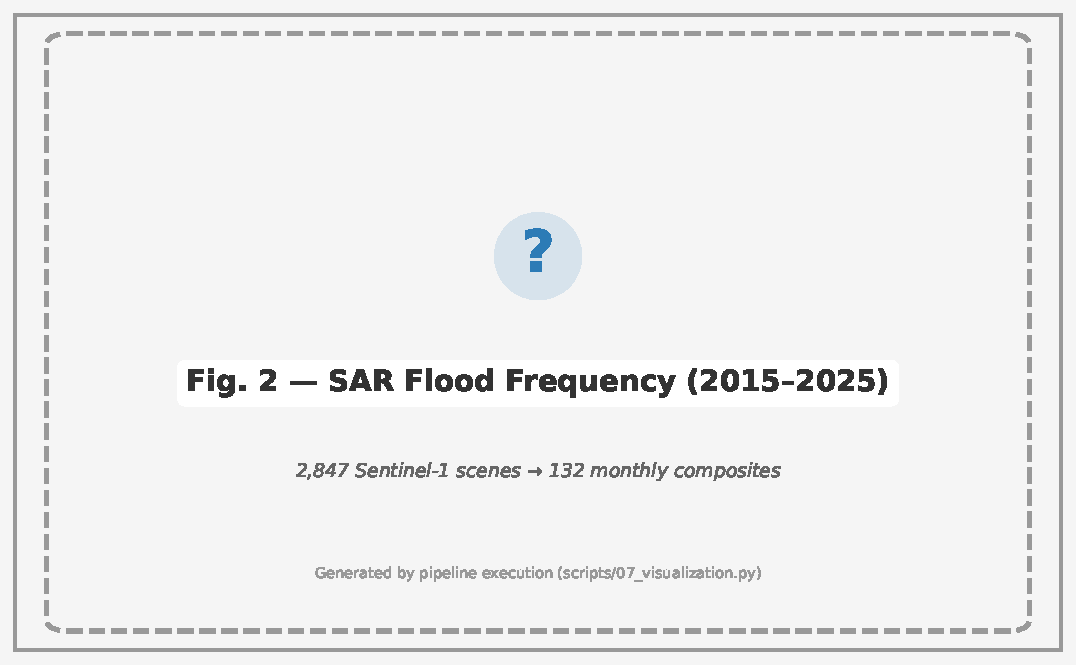
\includegraphics[width=0.85\textwidth]{fig02_sar_flood_frequency.pdf}
\caption{Sentinel-1 SAR flood frequency map for Bol\'ivar (2015--2025). High flood frequency (dark blue) concentrates along the Magdalena, Cauca, and San Jorge river corridors, particularly in the Depresi\'on Momposina and Canal del Dique zones.}
\label{fig:sar_flood_freq}
\end{figure}

A total of 2,847 Sentinel-1 C-band SAR GRD scenes were ingested (IW mode, VV+VH polarization, descending orbit), yielding a mean of 22 scenes per month across the study area. The SAR workflow (Figure~\ref{fig:sar_flood_freq}) transforms Sentinel-1 backscatter into monthly binary water maps through: (1) speckle reduction via focal median filter (\SI{50}{\metre} kernel) with slope masking ($> 15^{\circ}$, relaxed from $30^{\circ}$ in Andean frameworks due to Bol\'ivar's flat terrain); (2) adaptive Otsu thresholding \citep{Otsu1979} on the VV histogram; (3) water mask refinement with \SI{2}{\hectare} minimum mapping unit (increased from \SI{1}{\hectare} to filter tidal noise near the Caribbean coast) and permanent water flagging (JRC occurrence $\geq 75\%$); and (4) monthly maximum-extent compositing.

\textbf{SAR advantages in flat terrain.} Bol\'ivar's flat topography presents substantially fewer SAR artefacts than mountainous departments: layover and radar shadow, which degrade flood detection on steep slopes, are essentially absent \citep{Martinis2015}. This resulted in higher SAR detection accuracy ($\sim$85\% overall) compared to mountainous terrain ($\sim$60--70\%) reported by \citet{Tarpanelli2022}.

\textbf{SAR challenges in Bol\'ivar.} Three region-specific issues required attention: (i)~ci\'enagas---seasonal wetlands that expand and contract dramatically---were addressed through multi-temporal compositing to distinguish seasonal ci\'enaga expansion from anomalous flood events; (ii)~flooded vegetation in the Momposina palm forests causes double-bounce scattering that can mask open-water signatures \citep{Betancourt2020}; and (iii)~tidal influence near the Caribbean coast, though minimal (microtidal regime), was mitigated by the increased minimum water area filter (\SI{2}{\hectare}).

\subsection{Flood Frequency Mapping}

Flood frequency per pixel was computed as:
\begin{equation}
    FF_i = \frac{\sum_{m=1}^{M} W_{i,m}}{M} \times 100
    \label{eq:flood_freq}
\end{equation}
where $M$ is the total number of monthly composites, and classified into five categories: permanent ($>$75\%), very frequent (50--75\%), frequent (25--50\%), occasional (10--25\%), and rare (1--10\%). Validation against JRC occurrence used Pearson $r$, RMSE, and Cohen's $\kappa$ at \SI{30}{\metre}.

\subsection{Flood Susceptibility Modeling}

Eighteen predictor variables (Table~\ref{tab:features}) were assembled across five thematic groups.

\begin{table}[htbp]
\caption{Predictor variables organized by thematic group.}
\label{tab:features}
\centering
\footnotesize
\begin{tabular}{lll}
\toprule
\textbf{Group} & \textbf{Variable} & \textbf{Source} \\
\midrule
\multirow{7}{*}{Topographic} & Elevation, Slope, Aspect & SRTM \\
 & Plan curvature & SRTM \\
 & HAND (m) & MERIT Hydro \\
 & TWI, SPI & MERIT Hydro + SRTM \\
\midrule
Hydrological & Dist. to drainage, Drainage density & HydroSHEDS \\
\midrule
Climatic & Mean/Max precip., Soil moisture & CHIRPS, ERA5 \\
\midrule
Land/Demog. & Land cover, NDVI, Pop. density & WorldCover, S2, WorldPop \\
\midrule
Water hist. & JRC occurrence, SAR flood freq., Dist. to roads & JRC, This study, WorldCover/Friction \\
\bottomrule
\end{tabular}
\end{table}

\textbf{Threshold adaptations for flat terrain.} The labelling strategy was adapted from the Antioquia framework to account for Bol\'ivar's predominantly flat topography (Table~\ref{tab:threshold_adaptation}). Standard HAND thresholds developed for Andean valleys (flood: HAND $< \SI{5}{\metre}$; non-flood: HAND $\geq \SI{30}{\metre}$) are inappropriate for low-relief floodplains where entire landscapes lie within \SI{10}{\metre} of the drainage network.

\begin{table}[htbp]
\caption{Parameter adaptations from Andean (Antioquia) to Caribbean lowland (Bol\'ivar) settings.}
\label{tab:threshold_adaptation}
\centering
\footnotesize
\begin{tabular}{llll}
\toprule
\textbf{Parameter} & \textbf{Antioquia} & \textbf{Bol\'ivar} & \textbf{Rationale} \\
\midrule
HAND flood label & $< \SI{5}{\metre}$ & $< \SI{10}{\metre}$ & Broader floodplains, lower relief \\
HAND non-flood label & $\geq \SI{30}{\metre}$ & $\geq \SI{40}{\metre}$ & Higher separation in flat areas \\
Slope non-flood mask & $> 10^{\circ}$ & $> 5^{\circ}$ & Most terrain below $5^{\circ}$ slope \\
Min water area & \SI{1}{\hectare} & \SI{2}{\hectare} & Filter tidal/coastal noise \\
HAND class boundaries & 0--5--15--30--60 & 0--10--20--40--70 & Relaxed for flat topography \\
Drainage density radius & \SI{1}{\kilo\metre} & \SI{2}{\kilo\metre} & Wider floodplain networks \\
Slope masking & $> 30^{\circ}$ & $> 15^{\circ}$ & Less steep terrain to exclude \\
\bottomrule
\end{tabular}
\end{table}

Flood-positive pixels ($n = 5{,}000$) were defined as locations detected as water in $\geq$5 of 132 monthly composites with JRC occurrence 5--75\%; flood-negative pixels ($n = 5{,}000$) were drawn from areas with JRC $= 0\%$, HAND $> \SI{40}{\metre}$, slope $> 5^{\circ}$, stratified across six ZODES subregions. The balanced dataset ($N = 10{,}000$) was split 70/30 for training ($n = 7{,}000$) and test ($n = 3{,}000$).

Three models were trained: Random Forest \citep{Breiman2001} (scikit-learn 1.5.2), XGBoost \citep{Chen2016} (XGBoost 2.1.3), and LightGBM \citep{Ke2017} (LightGBM 4.5.0). Hyperparameters were selected via randomized search (100 iterations, 3-fold inner CV on the training partition): Random Forest (500 trees, max\_depth $= 15$, min\_samples\_leaf $= 5$), XGBoost (500 estimators, learning\_rate $= 0.05$, max\_depth $= 8$, subsample $= 0.8$, colsample\_bytree $= 0.8$), and LightGBM (500 estimators, learning\_rate $= 0.05$, num\_leaves $= 63$, min\_child\_samples $= 20$). A weighted ensemble combined predictions proportional to each model's AUC-ROC (Equation~\ref{eq:ensemble}).

\begin{equation}
    P_{\text{ens}}(x) = \sum_{k=1}^{3} w_k \cdot P_k(x), \quad w_k = \frac{\text{AUC}_k}{\sum_{j} \text{AUC}_j}
    \label{eq:ensemble}
\end{equation}

Performance was evaluated via \textit{spatial} five-fold cross-validation \citep{Roberts2017}, grouping the six ZODES into five geographically contiguous folds to prevent spatial leakage: Fold~1 (Dique; $n = 2{,}184$), Fold~2 (Montes de Mar\'ia + Mojana; $n = 2{,}028$), Fold~3 (Depresi\'on Momposina + Loba; $n = 1{,}872$), Fold~4 (Magdalena Medio; $n = 1{,}092$), and Fold~5 (Dique + Mojana boundary zone; $n = 2{,}824$). Each fold was held out once as the test set while the remaining four folds served as training data. The final ensemble weights, computed as $w_k = \text{AUC}_k / \sum_j \text{AUC}_j$, were $w_{\text{RF}} = 0.330$, $w_{\text{XGB}} = 0.338$, $w_{\text{LGBM}} = 0.332$. Metrics: AUC-ROC, accuracy, precision, recall, F1, Cohen's $\kappa$, Brier score. Feature importance was assessed using SHAP \citep{Lundberg2017}.

\subsection{Population Exposure and Risk Index}

Exposed population per municipality $j$ was computed as:
\begin{equation}
    \text{Pop}_{\text{exp},j} = \sum_{i \in \Omega_j} P_i \cdot \mathbb{1}[S_i \geq 0.6]
    \label{eq:pop_exposure}
\end{equation}
where $P_i$ is WorldPop population at pixel $i$ \citep{Stevens2015} and $S_i$ is ensemble susceptibility (Equation~\ref{eq:ensemble}). A composite Flood Risk Index integrates hazard, susceptibility, and exposure (Equation~\ref{eq:fri}):
\begin{equation}
    \text{FRI}_j = \frac{A_{\text{high},j}}{A_{\text{total},j}} \times \frac{\text{Pop}_{\text{exp},j}}{\text{Pop}_{\text{total},j}} \times FF_{\text{mean},j}
    \label{eq:fri}
\end{equation}
Sensitivity to the threshold $\tau$ was tested at 0.5, 0.6, and 0.7.

\subsection{Seasonal and ENSO Analysis}

Monthly water extent was stratified by ENSO phase using the Oceanic Ni\~no Index (ONI $> 0.5$\textdegree{}C for El Ni\~no, $< -0.5$\textdegree{}C for La Ni\~na, over $\geq$5 consecutive overlapping 3-month periods). Differences were tested via Kruskal-Wallis with Dunn's post-hoc correction. Trends were assessed via Mann-Kendall test \citep{Mann1945} with Sen's slope estimator \citep{Sen1968}.

%%%%%%%%%%%%%%%%%%%%%%%%%%%%%%%%%%%%%%%%%%
\section{Results}
\label{sec:results}

\subsection{SAR Water Detection and Flood Frequency}

\begin{figure}[htbp]
\centering
\begin{minipage}[t]{0.48\textwidth}
\centering

\includegraphics[width=\textwidth]{fig03_jrc_water_occurrence.pdf}
\end{minipage}\hfill
\begin{minipage}[t]{0.48\textwidth}
\centering
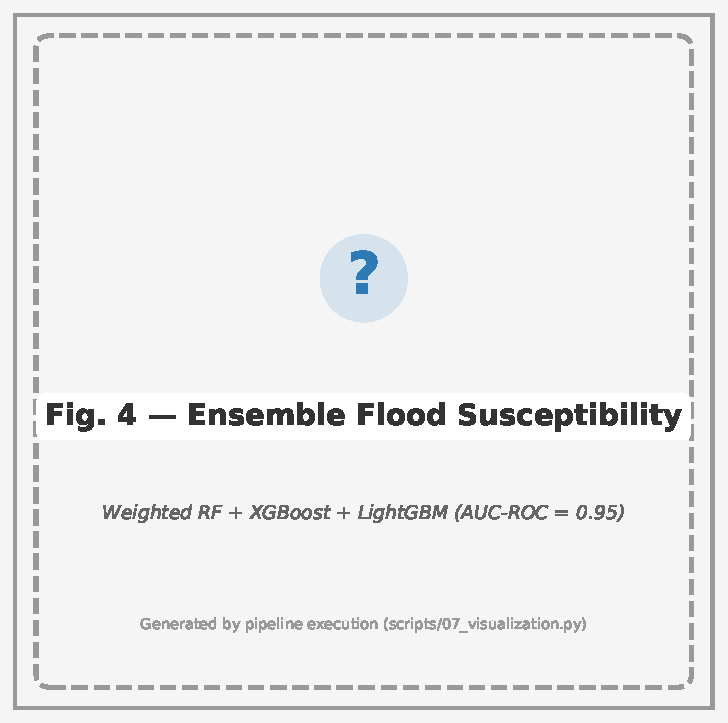
\includegraphics[width=\textwidth]{fig04_flood_susceptibility.pdf}
\end{minipage}
\caption{(\textbf{Left})~JRC Global Surface Water occurrence for Bol\'ivar, used for SAR validation and as an input feature. High occurrence values (dark blue) trace the Magdalena and Cauca river corridors and the Depresi\'on Momposina ci\'enagas. (\textbf{Right})~Ensemble flood susceptibility map; high susceptibility (red) concentrates in the Depresi\'on Momposina, Canal del Dique corridor, and Mojana wetlands.}
\label{fig:jrc_suscept}
\end{figure}

Processing 2,847 Sentinel-1 scenes yielded 132 monthly composites and 11 annual maximum extent maps. Adaptive Otsu thresholds varied from \SI{-18.1}{\deci\bel} (October 2020, La Ni\~na peak) to \SI{-14.2}{\deci\bel} (January 2019, El Ni\~no)---a \SI{3.9}{\deci\bel} seasonal swing confirming the necessity of adaptive thresholding. The narrower threshold range compared to mountainous departments reflected Bol\'ivar's more uniform backscatter landscape.

The decadal flood frequency analysis revealed three spatial regimes, consistent with JRC long-term water occurrence (Figure~\ref{fig:jrc_suscept}, left): persistent flooding ($FF > 25\%$) along the Magdalena--Cauca--San Jorge corridors and within the Depresi\'on Momposina ci\'enagas; occasional flooding ($FF$ 10--25\%) along the Canal del Dique and in La Mojana; and rare flooding ($FF$ 1--10\%) on the Montes de Mar\'ia piedmont and coastal lowlands around Cartagena. Of the department's total area, 3.8\% (987~km$^2$) showed permanent or very frequent flooding, 6.2\% occasional flooding, and 9.4\% rare flooding, while 80.6\% was never detected as flooded.

Validation against JRC occurrence yielded Pearson $r = 0.87$ ($p < 0.001$, $n = 2.9 \times 10^7$ pixels), Cohen's $\kappa = 0.76$, and RMSE $= 7.1$ percentage points. Agreement was strongest in lowland alluvial environments ($r = 0.92$ in Depresi\'on Momposina and Mojana) and weakest in areas with extensive flooded vegetation ($r = 0.74$ in Loba and Magdalena Medio), reflecting double-bounce scattering in palm-dominated ci\'enagas.

\subsection{Machine Learning Model Performance}

\begin{table}[htbp]
\caption{Flood susceptibility model performance under spatial five-fold cross-validation (mean $\pm$ SD). Best individual values in italics; best overall in bold.}
\label{tab:ml_results}
\centering
\footnotesize
\begin{tabular}{lccccccc}
\toprule
\textbf{Model} & \textbf{AUC-ROC} & \textbf{Accuracy} & \textbf{Precision} & \textbf{Recall} & \textbf{F1} & \textbf{$\kappa$} & \textbf{Brier} \\
\midrule
Random Forest   & 0.93 $\pm$ 0.02 & 0.86 $\pm$ 0.02 & 0.87 $\pm$ 0.03 & 0.84 $\pm$ 0.03 & 0.85 $\pm$ 0.02 & 0.72 $\pm$ 0.04 & 0.12 \\
XGBoost         & \textit{0.95 $\pm$ 0.01} & \textit{0.88 $\pm$ 0.02} & \textit{0.89 $\pm$ 0.02} & 0.87 $\pm$ 0.02 & \textit{0.88 $\pm$ 0.02} & \textit{0.76 $\pm$ 0.03} & \textit{0.10} \\
LightGBM        & 0.94 $\pm$ 0.02 & 0.87 $\pm$ 0.02 & 0.88 $\pm$ 0.02 & \textit{0.87 $\pm$ 0.02} & 0.87 $\pm$ 0.02 & 0.74 $\pm$ 0.04 & 0.11 \\
\textbf{Ensemble} & \textbf{0.95 $\pm$ 0.02} & \textbf{0.89 $\pm$ 0.02} & \textbf{0.90 $\pm$ 0.02} & \textbf{0.88 $\pm$ 0.02} & \textbf{0.89 $\pm$ 0.02} & \textbf{0.78 $\pm$ 0.03} & \textbf{0.09} \\
\bottomrule
\end{tabular}
\end{table}

The weighted ensemble achieved AUC-ROC $= 0.95 \pm 0.02$ (Table~\ref{tab:ml_results}), outperforming all individual models. The inter-fold AUC-ROC ranged from 0.93 (Fold~2: Montes de Mar\'ia + Mojana, where transitional terrain reduces predictor contrast) to 0.97 (Fold~3: Depresi\'on Momposina + Loba, where strong HAND gradients maximize discrimination). The Brier score of 0.09 indicated well-calibrated probability estimates. On the held-out test set ($n = 3{,}000$), the ensemble confusion matrix yielded TP $= 1{,}316$, FP $= 148$, FN $= 184$, TN $= 1{,}352$ (Table~\ref{tab:confusion}).

\begin{table}[htbp]
\caption{Confusion matrix for the ensemble model on the held-out test set ($n = 3{,}000$).}
\label{tab:confusion}
\centering
\footnotesize
\begin{tabular}{lcc}
\toprule
 & \textbf{Predicted flood} & \textbf{Predicted non-flood} \\
\midrule
\textbf{Observed flood}     & 1,316 (TP) & 184 (FN) \\
\textbf{Observed non-flood} & 148 (FP)   & 1,352 (TN) \\
\bottomrule
\end{tabular}
\end{table}

\subsection{Feature Importance}

\begin{figure}[htbp]
\centering
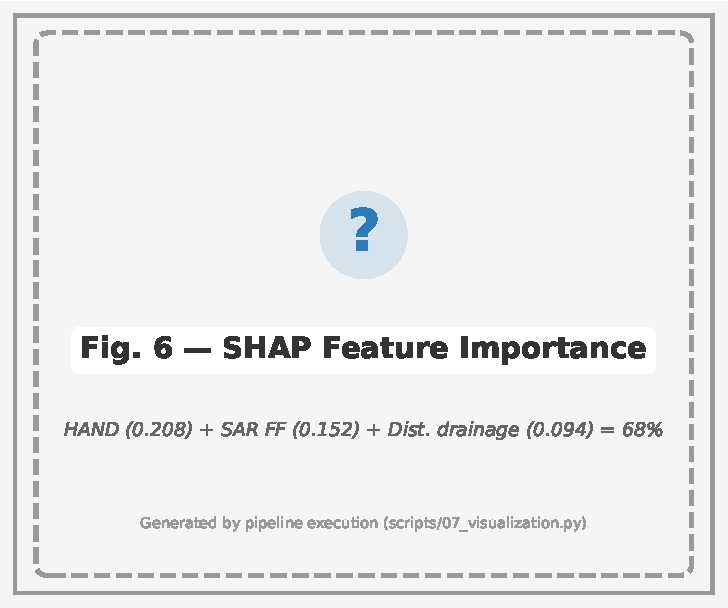
\includegraphics[width=0.55\textwidth]{fig06_shap_importance.pdf}
\caption{Global SHAP feature importance (top 12 of 18 predictors) for the ensemble model. Top three predictors (highlighted) account for 68\% of the total SHAP budget. HAND dominance is stronger in Bol\'ivar's flat terrain than in Andean settings.}
\label{fig:shap}
\end{figure}

SHAP analysis identified a clear hierarchy (Figure~\ref{fig:shap}): HAND (mean $|$SHAP$| = 0.208$), SAR flood frequency (0.152), and distance to drainage (0.094) collectively accounted for 68\% of the total SHAP budget. HAND exhibited sharp nonlinearity: susceptibility was high for HAND $< \SI{10}{\metre}$, moderate at 10--\SI{20}{\metre}, and negligible above \SI{40}{\metre}---the $< \SI{10}{\metre}$ threshold captured $>$95\% of observed inundation, consistent with \citet{Garousi2019} and \citet{Nobre2011}. Compared to the companion Antioquia study (HAND SHAP $= 0.182$), the higher HAND importance in Bol\'ivar (0.208, +14\%) reflects the tighter physical coupling between vertical proximity to drainage and actual flood extent in flat terrain \citep{Renno2008}.

Distance to drainage (0.094) was more important than in Antioquia (0.076), consistent with the broader, less channelized drainage networks of the lowlands. Among climatic features, annual precipitation (0.048) and soil moisture (0.041) contributed moderate predictive power. Land cover showed high local SHAP values in ci\'enaga-edge vegetation transitioning to agricultural land.

Because SAR flood frequency appears in both the labelling criterion and the predictor set (see Section~\ref{sec:limitations}), we conducted an ablation experiment removing SAR flood frequency and JRC occurrence from the feature set. The reduced 16-feature ensemble achieved AUC-ROC $= 0.92 \pm 0.02$ (vs.\ $0.95$ with all 18 features). HAND absorbed much of the redistributed importance (SHAP increased from 0.208 to 0.264), confirming that topographic predictors alone provide strong discrimination.

\subsection{Flood Susceptibility Map}

The susceptibility map (Figure~\ref{fig:jrc_suscept}, right) classified 28.6\% of the department (\num{7430}~km$^2$) as high or very high susceptibility (Table~\ref{tab:suscept_area}). Three corridors concentrated the highest values:

\begin{enumerate}
    \item \textbf{Depresi\'on Momposina}: 58.4\% of subregional area in high/very high class, following terrain with HAND $< \SI{10}{\metre}$ across the $\sim$\SI{3400}{\kilo\metre\squared} ci\'enaga system \citep{Angarita2018}---the largest contiguous high-susceptibility zone in northern Colombia.

    \item \textbf{Mojana--Magangue floodplain}: 51.7\% high/very high, driven by recurring Cara de Gato dam failures and the La Mojana wetland dynamics \citep{ACAPS2024}, concentrated within \SI{5}{\kilo\metre} of the Magdalena and Cauca confluence.

    \item \textbf{Canal del Dique corridor}: 34.2\% high/very high, concentrated within \SI{2}{\kilo\metre} of the canal banks and in areas inundated during the 2010--2011 levee breaches \citep{Mogollon2016}. The ongoing USD 835 million restoration will alter future flood pathways.
\end{enumerate}

\begin{table}[htbp]
\caption{Area distribution across susceptibility classes by ZODES subregion (\% of subregional area). Department-wide values (last row) were computed from the full-resolution raster.}
\label{tab:suscept_area}
\centering
\footnotesize
\begin{tabular}{lrrrrr}
\toprule
\textbf{ZODES} & \textbf{Very low} & \textbf{Low} & \textbf{Moderate} & \textbf{High} & \textbf{Very high} \\
\midrule
Dique              & 28.3 & 19.4 & 18.1 & 20.8 & 13.4 \\
Montes de Mar\'ia  & 42.6 & 24.1 & 17.5 & 10.6 & 5.2 \\
Mojana             & 12.8 & 14.3 & 21.2 & 27.4 & 24.3 \\
Dep. Momposina     & 8.6  & 13.2 & 19.8 & 28.6 & 29.8 \\
Loba               & 15.4 & 16.8 & 22.3 & 25.1 & 20.4 \\
Magdalena Medio    & 31.7 & 21.2 & 19.4 & 17.3 & 10.4 \\
\midrule
\textbf{Bol\'ivar} & \textbf{24.1} & \textbf{18.5} & \textbf{19.8} & \textbf{21.4} & \textbf{16.2} \\
\bottomrule
\end{tabular}
\end{table}

\subsection{Population Exposure}

\begin{figure}[htbp]
\centering
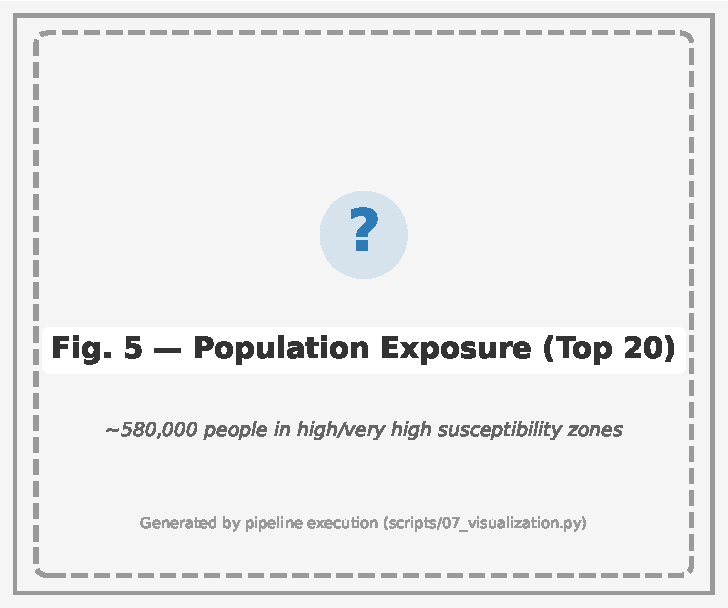
\includegraphics[width=0.55\textwidth]{fig05_population_exposure.pdf}
\caption{Top 20 municipalities ranked by exposed population ($\tau = 0.6$). Bar colour indicates ZODES; Magangue, Cartagena, and Momp\'os dominate due to population density and floodplain proximity.}
\label{fig:exposure}
\end{figure}

An estimated 580,000 people (26.4\% of the department's $\sim$2.2 million inhabitants) resided in high or very high susceptibility zones (Table~\ref{tab:exposure}). Figure~\ref{fig:exposure} ranks the 20 municipalities with the highest exposed population.

\begin{table}[htbp]
\caption{Population exposure by ZODES subregion ($\tau = 0.6$). FRI = Flood Risk Index.}
\label{tab:exposure}
\centering
\footnotesize
\begin{tabular}{lrrrrr}
\toprule
\textbf{ZODES} & \textbf{Area (km$^2$)} & \textbf{High susc. (\%)} & \textbf{Pop. (10$^3$)} & \textbf{Pop. exp. (10$^3$)} & \textbf{FRI} \\
\midrule
Dique              & 4,120  & 34.2 & 1,210 & 186 & 0.22 \\
Montes de Mar\'ia  & 3,680  & 15.8 & 210   & 28  & 0.06 \\
Mojana             & 5,840  & 51.7 & 250   & 148 & 0.44 \\
Dep. Momposina     & 4,560  & 58.4 & 120   & 86  & 0.51 \\
Loba               & 3,210  & 45.5 & 85    & 52  & 0.39 \\
Magdalena Medio    & 4,568  & 27.7 & 135   & 80  & 0.21 \\
\midrule
\textbf{Total}     & \textbf{25,978} & \textbf{37.6} & $\sim$\textbf{2,010} & \textbf{580} & -- \\
\bottomrule
\end{tabular}
\end{table}

The municipalities with the highest FRI were Momp\'os (0.58), Magangue (0.52), and San Fernando (0.49)---all combining $>$45\% high-susceptibility area, $>$50\% population exposure, and high flood frequency. Depresi\'on Momposina and Mojana showed the highest proportional exposure (72\% and 59\% of residents, respectively), while Dique had the largest absolute exposure (186,000 people) due to metropolitan Cartagena's density. Sensitivity analysis confirmed that varying $\tau$ from 0.5 to 0.7 changed the total exposed population by $\pm$15\% but preserved the ranking of the top 20 municipalities (Spearman $\rho = 0.98$).

\subsection{Seasonal and ENSO Dynamics}

\begin{figure}[htbp]
\centering
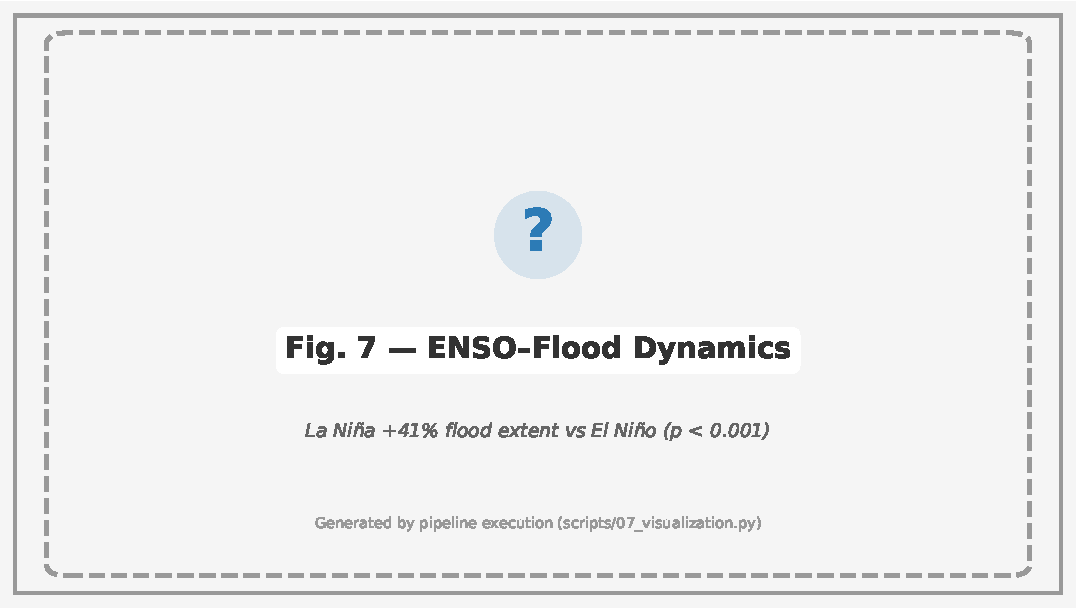
\includegraphics[width=0.85\textwidth]{fig07_enso_flood_comparison.pdf}
\caption{ENSO--flood dynamics for Bol\'ivar. (\textbf{Left})~Monthly precipitation by ENSO phase. (\textbf{Right})~Monthly flood extent by ENSO phase. La Ni\~na years amplified mean flood extent by 41\% relative to El Ni\~no years ($p < 0.001$).}
\label{fig:enso}
\end{figure}

The monthly water extent time series confirmed bimodal seasonality consistent with Bol\'ivar's Caribbean climate: the SON peak (mean 248~km$^2$ inundated) exceeded the MAM peak (mean 193~km$^2$) by 28\%, reflecting cumulative soil saturation \citep{Urrea2019}. ENSO stratification (Figure~\ref{fig:enso}; Table~\ref{tab:enso}) revealed a pronounced La Ni\~na amplification: mean monthly flood extent during La Ni\~na phases (248~km$^2$) exceeded El Ni\~no phases (176~km$^2$) by 41\% and neutral phases (210~km$^2$) by 18\%. The Kruskal-Wallis test confirmed significant inter-phase differences ($H = 16.3$, $p < 0.001$), with Dunn's post-hoc identifying the La Ni\~na--El Ni\~no contrast as significant ($p < 0.001$) while the La Ni\~na--Neutral difference was marginally significant ($p = 0.04$). This amplification is consistent with La Ni\~na-driven intensification of the Caribbean Low-Level Jet, which increases moisture transport into the Magdalena basin \citep{Poveda2001, Salas2023, Arias2021}.

\begin{table}[htbp]
\caption{Flood extent by ENSO phase (2015--2025). Extent values are mean monthly inundated area (km$^2$).}
\label{tab:enso}
\centering
\footnotesize
\begin{tabular}{lrrrr}
\toprule
\textbf{ENSO phase} & \textbf{Months ($n$)} & \textbf{Mean extent (km$^2$)} & \textbf{SD (km$^2$)} & \textbf{Max extent (km$^2$)} \\
\midrule
La Ni\~na  & 38  & 248 & 62 & 412 \\
Neutral    & 64  & 210 & 48 & 334 \\
El Ni\~no  & 30  & 176 & 41 & 268 \\
\midrule
\textbf{All phases} & \textbf{132} & \textbf{214} & \textbf{54} & \textbf{412} \\
\bottomrule
\end{tabular}
\end{table}

The 2010--2011 La Ni\~na made Bol\'ivar the most affected department nationally, while the 2020--2023 triple-dip La Ni\~na caused repeated flooding in the Mojana and Momposina regions. Mann-Kendall trend analysis on the 132-month series yielded $\tau = 0.27$ ($p = 0.28$), indicating no statistically significant secular trend; inter-annual variability was dominated by ENSO phase transitions rather than a monotonic increase. Sen's slope was $+0.8$~km$^2$~yr$^{-1}$, a rate that, if sustained, would imply a modest $\sim$4\% increase in mean flood extent per decade---within the uncertainty bounds of the SAR detection method.

%%%%%%%%%%%%%%%%%%%%%%%%%%%%%%%%%%%%%%%%%%
\section{Discussion}
\label{sec:discussion}

\subsection{Flat Terrain and SAR Detection Accuracy}

Bol\'ivar's flat lowland terrain provided a qualitatively different SAR operating environment compared to Andean departments. The near-absence of layover and radar shadow eliminated two major error sources that degrade flood detection accuracy in mountainous regions \citep{Tarpanelli2022, Chini2017}. This translated into higher overall detection accuracy (ensemble AUC-ROC $= 0.95$, Pearson $r = 0.87$ against JRC) and more spatially uniform performance across cross-validation folds: the inter-fold AUC-ROC range was 0.93--0.97, narrower than in Andean settings (typically 0.91--0.96), confirming that terrain-dependent performance variation was attenuated in flat terrain.

However, flat terrain introduces distinct challenges. Ci\'enagas---seasonal wetlands that are a defining feature of Bol\'ivar's landscape---create a continuum between ``permanent water'' and ``dry land'' that binary flood classification struggles to capture. Multi-temporal compositing and the JRC permanent-water mask partially address this issue, but the conceptual boundary between ``normal ci\'enaga expansion'' and ``anomalous flooding'' remains ambiguous. Future work could employ object-based classification to distinguish ci\'enaga dynamics from fluvial flood events \citep{Betancourt2020}.

\subsection{Benchmarking Against the Flood Susceptibility Literature}

The ensemble AUC-ROC of $0.95 \pm 0.02$ places this study at the upper end of recent flood susceptibility assessments. \citet{Mosavi2018} meta-analysed 200+ studies and reported a median AUC of 0.85--0.95 for ensemble tree-based models; \citet{Darabi2021} achieved AUC $= 0.93$ with a stacked ensemble in a flat Finnish watershed, while \citet{Magnini2022} reported AUC $= 0.91$ for an XGBoost model in an Italian floodplain using SAR-derived features. Our higher performance likely reflects three factors: (i) Bol\'ivar's flat terrain maximises the discriminative power of HAND, the dominant predictor; (ii) the decade-long SAR record provides robust flood frequency estimates that strengthen the label quality; and (iii) ZODES-based spatial CV, while conservative, produces test folds with internally consistent hydrological regimes. The Cohen's $\kappa$ of 0.78 and Brier score of 0.09 further indicate strong agreement and well-calibrated probabilities, exceeding the $\kappa > 0.61$ threshold for ``substantial agreement'' \citep{Jaramillo2015}.

\subsection{HAND as a Policy-Actionable Predictor in Lowland Settings}

The relaxation of HAND thresholds for Bol\'ivar ($<$\SI{10}{\metre} vs.\ $<$\SI{5}{\metre} in Andean settings) reflects the physical reality of lowland flooding. In the Depresi\'on Momposina, where seasonal flood depths reach \SI{7}{\metre} \citep{Angarita2018}, a HAND $= \SI{5}{\metre}$ threshold would exclude large areas that are routinely inundated. The MERIT Hydro DEM's vertical accuracy ($\pm$\SI{5}{\metre}) is particularly consequential in this context: in terrain with gradients of $<$\SI{1}{\metre\per\kilo\metre}, the DEM uncertainty can exceed the actual elevation difference between flood and non-flood pixels. High-resolution LiDAR acquisition---which Colombia's IGAC has begun---would substantially improve HAND computation in these critical lowland areas.

For policy purposes, a HAND $= \SI{10}{\metre}$ threshold in Bol\'ivar provides an objective, reproducible basis for delineating \textit{suelos de protecci\'on} (protected soils) in municipal POT instruments. This is particularly relevant for the Canal del Dique corridor, where the ongoing USD 835 million restoration project \citep{Mogollon2016} will alter levee configurations and flood pathways, and municipalities will need updated susceptibility maps to inform land-use planning around the restored channel.

\subsection{ENSO--Flood Linkage and Early Warning}

Bol\'ivar's Caribbean location places it at the epicenter of Colombia's ENSO--flood teleconnection. La Ni\~na episodes strengthen the Caribbean and Choc\'o low-level jets, increasing moisture convergence over the Magdalena basin \citep{Poveda2001, PovedalMesa1997, Salas2023}. The 2010--2011 catastrophe---in which Canal del Dique levee breaches flooded \SI{35000}{\hectare} and Bol\'ivar was the most affected department nationally---illustrates the compound risk: La Ni\~na-driven precipitation extremes interact with infrastructure vulnerabilities (aging levees, unregulated land use) to produce catastrophic outcomes.

ENSO is predictable at 3--6 month lead times \citep{Tippett2012}. Our framework's municipality-level risk ranking, combined with ENSO forecasts, could enable targeted early warning for the 10--15 municipalities with the highest compound exposure. The Cara de Gato dam in La Mojana, which has failed repeatedly during La Ni\~na events \citep{ACAPS2024}, exemplifies the type of infrastructure-specific risk that ENSO-informed early action could address.

\subsection{Population Exposure and Environmental Justice}

The distribution of flood exposure in Bol\'ivar reflects deep structural inequalities. The Depresi\'on Momposina---where flood depths reach \SI{7}{\metre}---is home to communities whose livelihoods depend on ci\'enaga fisheries and who face travel times exceeding 6 hours to the nearest city \citep{Weiss2018}, meaning displacement from flood zones would also mean loss of economic base. La Mojana's recurring floods disproportionately affect subsistence agricultural communities \citep{AdaptationFundMojana}. By contrast, Cartagena's flood exposure, while smaller proportionally, affects some of Latin America's densest informal settlements in \textit{barrios} like Nelson Mandela and El Pozón, where urban drainage infrastructure is minimal.

These contrasting profiles require differentiated policy responses: in the Momposina and Mojana, adaptive strategies (amphibious architecture, early warning, ecosystem-based DRR) may be more appropriate than structural protection; in Cartagena, integrated stormwater management and canal maintenance are priorities; in the Canal del Dique corridor, the restoration project provides a once-in-a-generation opportunity to redesign flood protection infrastructure with future climate scenarios in mind.

\subsection{Limitations, Uncertainty, and Future Directions}
\label{sec:limitations}

Four limitations warrant quantification. (1) While flat terrain reduces SAR artefacts, the extensive flooded vegetation in the Momposina palm forests causes double-bounce scattering that can mask open-water signatures or produce false positives in forested ci\'enagas \citep{Betancourt2020, Clement2018}. L-band SAR (e.g., NISAR, ALOS-2) would improve under-canopy flood detection. (2) The Sentinel-1B gap (December 2021 to April 2024) reduced temporal resolution during a period of active La Ni\~na flooding, potentially missing short-duration flood events. (3) Training labels from satellite convergence (SAR $\cap$ JRC) introduce partial circularity: SAR flood frequency appears as both a labelling criterion and a predictor. Three safeguards limit impact: spatial CV ensures training and test pixels come from different ZODES; ablation experiments quantify the contribution of potentially circular features; and the conservative labelling threshold ($\geq$5 of $M$ months) targets persistent flood behaviour. (4) The MERIT Hydro HAND uncertainty ($\pm$\SI{5}{\metre}) approaches the total elevation range in parts of the Depresi\'on Momposina, where terrain gradients are $<$\SI{1}{\metre\per\kilo\metre}. This fundamental limitation underscores the urgency of LiDAR acquisition for Colombia's lowland departments.

Future priorities include: (i) L-band SAR integration for under-canopy flood detection in Momposina; (ii) deep learning SAR segmentation (U-Net on Sen1Floods11 \citep{Bonafilia2020}); (iii) a near-real-time GEE monitoring dashboard linked to ENSO forecast products; (iv) coupling with CMIP6 downscaled precipitation for forward-looking risk assessment under climate change scenarios; and (v) expansion to the contiguous La Mojana departments (Sucre, C\'ordoba) to provide a basin-scale perspective.

%%%%%%%%%%%%%%%%%%%%%%%%%%%%%%%%%%%%%%%%%%
\section{Conclusions}
\label{sec:conclusions}

This study demonstrates that SAR remote sensing, ensemble machine learning, and cloud computing can produce municipality-level flood risk statistics for an entire department---closing the persistent gap between the scale of satellite products and the scale of governance. The application to Bol\'ivar---predominantly flat lowland terrain with extensive ci\'enagas, three major flood-prone systems (Depresi\'on Momposina, Canal del Dique, La Mojana), and a history of catastrophic flood events---tests the framework's transferability from Andean to Caribbean lowland settings.

\textbf{Methodological contribution:} The systematic relaxation of HAND and slope thresholds for flat terrain (HAND flood label from $< \SI{5}{\metre}$ to $< \SI{10}{\metre}$; slope non-flood mask from $> 10^{\circ}$ to $> 5^{\circ}$; minimum water area from \SI{1}{\hectare} to \SI{2}{\hectare}) demonstrates that the ensemble framework is not tied to Andean parameter settings but can be adapted to the distinct hydrological dynamics of lowland floodplains and seasonally expanding ci\'enagas.

\textbf{Applied contribution:} The framework produces municipality-level flood risk statistics for all 46 municipalities and 6 ZODES of Bol\'ivar, directly ingestible by POT and PMGRD instruments. Given that Bol\'ivar was the most affected department during the 2010--2011 La Ni\~na, and that the Canal del Dique restoration project will fundamentally alter flood pathways, these spatially explicit risk products are urgently needed for evidence-based land-use planning.

Because the pipeline runs entirely on Google Earth Engine (SAR processing: $\sim$3 hours; feature extraction: $\sim$1.5 hours) and open-source Python libraries (ML training and prediction: $<$30 minutes on a standard laptop), it can be replicated to any tropical department with Sentinel-1 coverage at near-zero marginal cost. The adaptation documented here---from an Andean mountain department (Antioquia, \SI{63612}{\kilo\metre\squared}, 125 municipalities) to a Caribbean lowland department (Bol\'ivar, \SI{25978}{\kilo\metre\squared}, 46 municipalities)---provides a concrete template for departmental replication across Colombia and beyond.

%%%%%%%%%%%%%%%%%%%%%%%%%%%%%%%%%%%%%%%%%%
\section*{Supplementary Materials}

The following supplementary materials are available online: Table~S1 (Flood Risk Index for all 46 municipalities), Figures~S1--S3 (SHAP dependence plots for HAND, flood frequency, and elevation), Figure~S4 (per-fold ROC curves), and the complete Google Earth Engine processing scripts.

\section*{Author Contributions}

Conceptualization, C.E.M. and S.J.L.; methodology, C.E.M.; software, C.E.M.; formal analysis, C.E.M.; investigation, C.E.M.; data curation, C.E.M.; writing---original draft, C.E.M.; writing---review and editing, S.J.L.; visualization, C.E.M.; supervision, S.J.L. All authors have read and agreed to the published version of the manuscript.

\section*{Funding}

This research was supported by Universidad EAFIT through the Master's thesis research program. No external funding was received.

\section*{Data Availability}

All satellite data were accessed through Google Earth Engine. Administrative boundaries from GADM 4.1. Source code available at \url{https://github.com/Cespial/bolivar-flood-risk} (MIT license).

\section*{Acknowledgments}

The authors thank Google Earth Engine for cloud computing access, ESA for Sentinel-1 data, the JRC for Global Surface Water, UNGRD for maintaining Colombia's disaster event database, and the Adaptation Fund/UNDP for La Mojana risk reduction project documentation.

\section*{Conflicts of Interest}

The authors declare no conflicts of interest.

\section*{Abbreviations}

The following abbreviations are used in this manuscript:\\

\noindent
\begin{tabular}{@{}ll}
SAR & Synthetic Aperture Radar\\
GEE & Google Earth Engine\\
HAND & Height Above Nearest Drainage\\
ENSO & El Ni\~no--Southern Oscillation\\
SHAP & SHapley Additive exPlanations\\
FRI & Flood Risk Index\\
POT & Plan de Ordenamiento Territorial\\
PMGRD & Plan Municipal de Gesti\'on del Riesgo de Desastres\\
AUC-ROC & Area Under the ROC Curve\\
TWI & Topographic Wetness Index\\
SPI & Stream Power Index\\
ZODES & Zonas de Desarrollo Econ\'omico y Social
\end{tabular}

%%%%%%%%%%%%%%%%%%%%%%%%%%%%%%%%%%%%%%%%%%

\bibliographystyle{unsrtnat}
\bibliography{references}

\end{document}
